\chapter{Evolutionary Generation of Swarm Algorithms}
\label{ch:EvolutionaryGeneration}

\section{Introduction}

Swarms are complex systems whose behavior is difficult to determine \apriori{} regardless of the predictive measures used.  Although some recent progress has been made on mathematical analysis of certain swarm algorithms~\cite{
couzin:CollectiveMemory, 
fax:InformationFlow, 
gazi:SwarmStability, 
grunbaum:InteractiveSwarms, 
huepe:ParticleClustering, 
jadbabaie:Coordination, 
marshall:VehicleFormations, 
paley:CollectiveMotion, 
parrish:FishSchools, 
toner:QuantitativeFlocking,
topaz:SwarmingPatterns, 
vicsek:PhaseTransition}, the full simulation of a swarm algorithm is currently the best known method of evaluating both the expected and emergent behaviors of the algorithm.  Thus, it is not surprising to find that the current state of the art in swarm algorithm development is primarily relegated to a trial-and-error methodology.  The realization of desired high-level behaviors for a swarm without the need to define and program the necessary lower-level behaviors would be an invaluable tool to both programmers and non-programmers alike.  

This chapter describes the development of \ECS (Evolutionary Computing for Swarms), an evolutionary computation engine designed to evolve swarm behavior algorithms.  The overall goal of \ECS is the realization of an evolutionary computing architecture that is capable of automatically generating swarm algorithms that exploit the inherent emergent properties of swarms with minimal user interaction.

\section{System Overview}

\refFigure{SystemOverview} is a conceptual overview of \ECS.  The system is a composition of a component-based evolutionary computing framework and the \SWEEP swarm algorithm simulator.  From a high-level perspective, \ECS operates similarly to a traditional evolutionary computing system~\cite{jholland:Adaptation}.  An initial population of candidate solutions, represented as finite state machines, are randomly generated.  Each  solution in the population is then evaluated using \SWEEP, resulting in a fitness score for each solution.  The next generation of the population is produced through the application of reproduction and mutation operators on individual solutions selected by criteria such as relative fitness or random selection.  Finally, the entire evaluate-reproduce cycle is repeated until a solution is found that satisfies the termination criteria.  \refAlgorithm{ECS} is a pseudo-code representation of basic execution flow of \ECS{}.

\begin{figure}[ht]
  \centering
  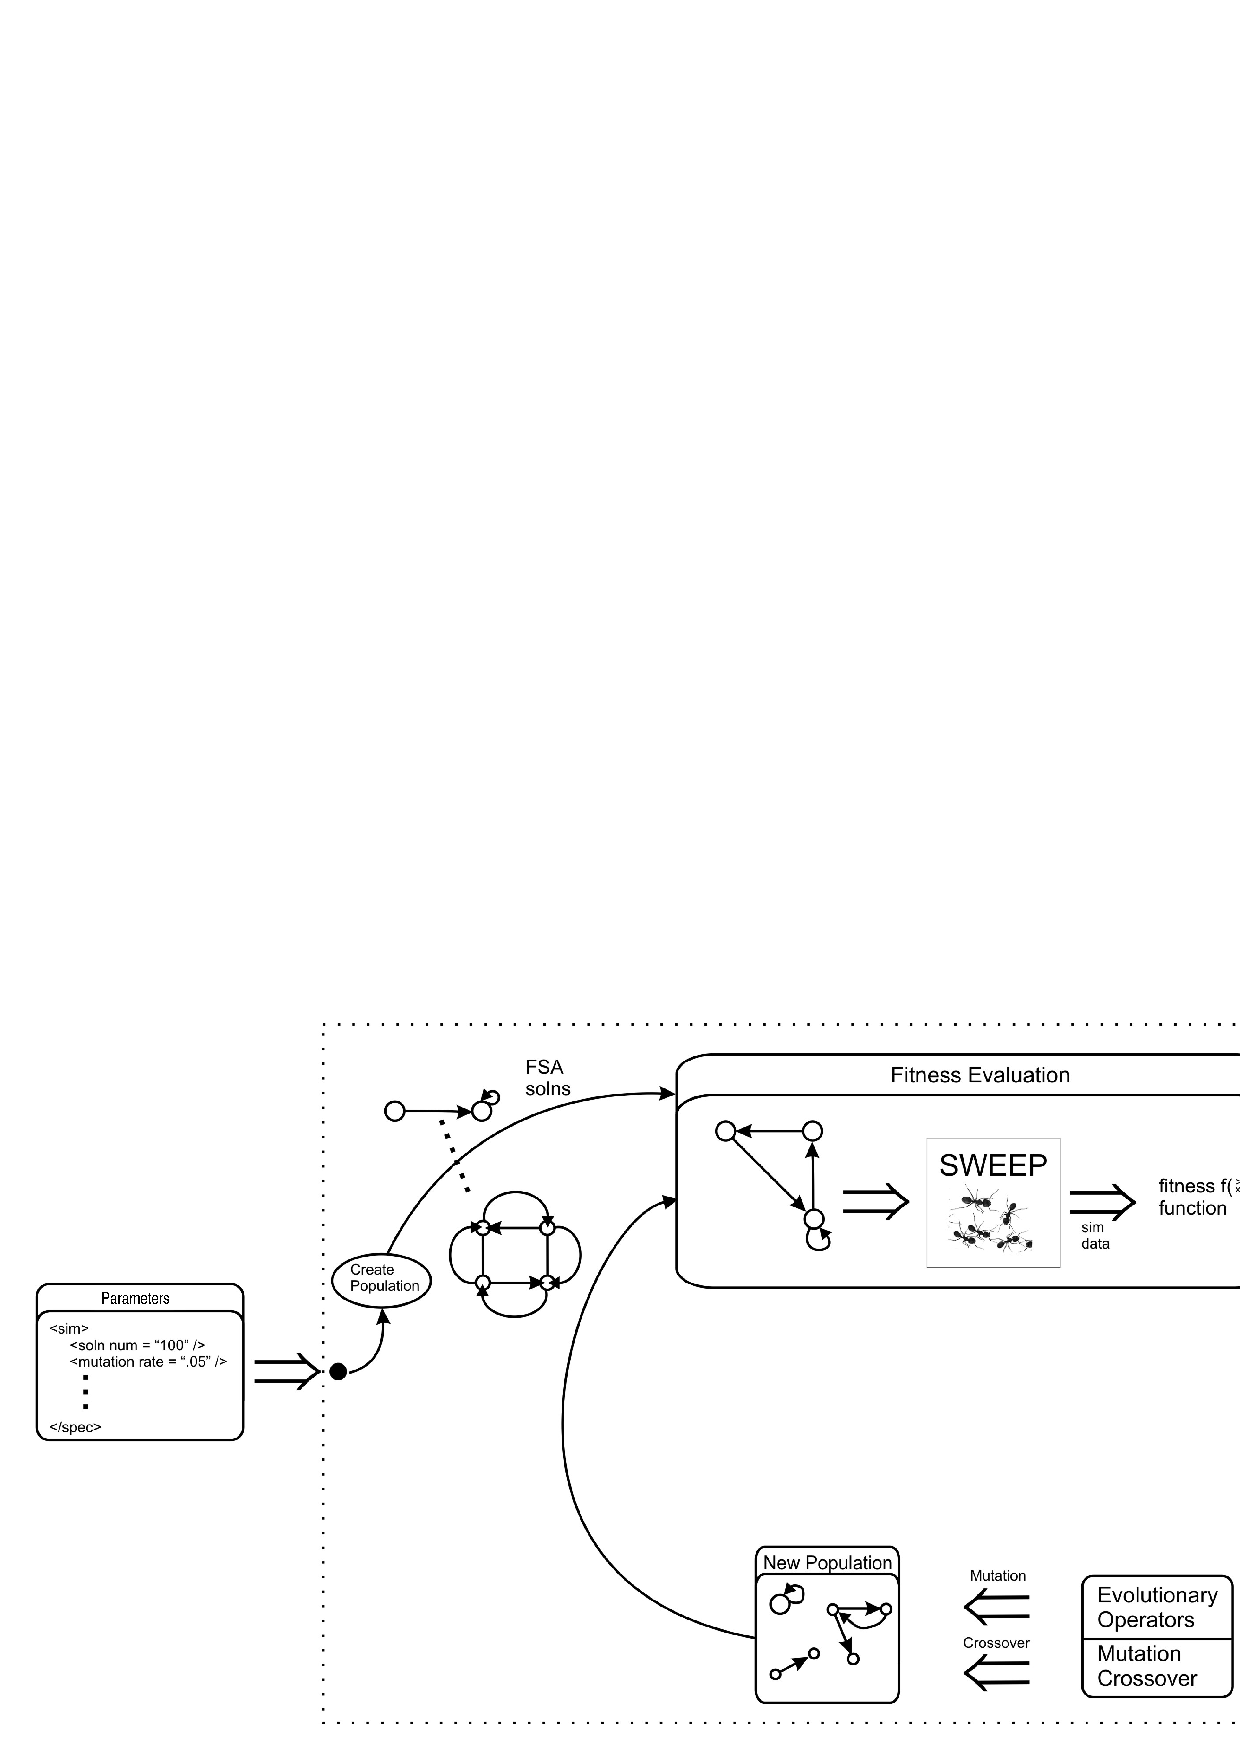
\includegraphics[width=.91\textwidth]{Figures/SystemOverview.pdf}
  \caption{Conceptual overview of \ECS (\ECSexp).}
  \label{fig:SystemOverview}
\end{figure}	

\begin{algorithm}[ht]
  \caption{Pseudo-code for the basic functionality of \ECS{}}
  \label{alg:ECS}
  \begin{algorithmic}[1]
    \REQUIRE isValid(parameters.xml)
    
    \STATE initialize(parameters.xml)
    \STATE mutations = generateMutations()
    \STATE sweep = createSWEEP()	
    \STATE population = generatePopulation()
    \STATE gen  $\leftarrow$ 0
    \STATE done $\leftarrow$ \false{}
    
    \WHILE{ $\neg$done }
    \STATE population = population $\cup$ createRandomSolution() 
    \COMMENT{Helps prevent homogenization}
    
    \FORALL{$m$ in mutations}
    \STATE population = population $\cup$ $m$.selectAndMutate()
    \ENDFOR
    
    \FORALL{$x$ in population}
    \STATE sweep.eval($x$)
    \ENDFOR
    
    \IF{$\exists x \in$ population such that isSolution($x$) == $\true{}$} 
    \STATE done $\leftarrow \true{}$
    \ENDIF
    
    \STATE gen $\leftarrow$ gen $+ 1$
    
    \IF{gen $\geq$ max\_generations}
    \STATE done $\leftarrow \true{}$
    \ENDIF
    \ENDWHILE
  \end{algorithmic}
\end{algorithm}

\section{System Parameters}
\label{sec:system-parameters}

\ECS{} has many configurable parameters that must be set in order to function.  \refTable{ExampleParameters} shows a sample set of parameters for evolving a dispersion algorithm.  The \italic{Objective} exists for documentation purposes and is a short description of the behavior that is being evolved.  \italic{Maximum Generations} specifies the upper limit on the number of generations that \ECS{} can execute before terminating execution.  The \italic{Population Size} specifies both the number of candidate solutions to initially create and the number of solutions that will be allowed to survive between generations as selected through elitism.  Finally, the \italic{Number of Simulations} indicates the number of \SWEEP{} simulations to average over when calculating fitness scores.  

Each mutation is applied a specific number of times each generation.  The resulting mutated solutions are then rolled back into the population to compete for survival.  When specifying how to apply a mutation, a selection method and selection size must be specified.  Currently \ECS{} supports \italic{random selection}, \italic{elite selection} (which selects the top $n$ solutions), and \italic{roulette selection} (which selects solutions randomly in proportion to their fitness relative to all other solutions)~\cite{back:ec1}.

The specified \italic{Actions} and \italic{Sensors} are the primary components used to build candidate solutions.  Any valid \SWEEP{} \italic{Action} or \italic{Sensor} is able to be included.  Currently, no validity checking is performed to ensure the compatibility of the \italic{Actions} and \italic{Sensors}.

Finally, the parameters related to simulating the candidate solutions with \SWEEP{} are specified.  The number and type of parameters will vary based on the simulations needs of the fitness function used.  In this case, the swarm size, environment size, and maximum number of time steps are specified.  

\begin{table}[ht]
  \centering
  \begin{tabular}{|lc|}
    \hline
    \multicolumn{2}{|c|}{\em{Parameters}} \\
    Objective & Dispersion \\
    Max. Generations & 500 \\
    Population Size & 73 \\
    Number of Trials & 2 \\	
    \hline
    \hline
    \multicolumn{2}{|c|}{\em{Mutations}}   \\
    Change-Sensor-Value & top 6 + 2 random \\
    Change-Next-State   & top 6 + 2 random \\
    Add-Transition      & top 6 + 2 random \\
    \hline
    \hline
    \multicolumn{2}{|c|}{\em{Actions}} \\
    \multicolumn{2}{|c|}{move-random} \\
    \multicolumn{2}{|c|}{move-none} \\
    \hline
    \multicolumn{2}{|c|}{\em{Sensors}} \\
    \multicolumn{2}{|c|}{neighbor-left} \\
    \multicolumn{2}{|c|}{neighbor-right} \\
    \hline
    \hline
    \multicolumn{2}{|c|}{\em{Simulation}} \\
    Number of Agents & 100 \\
    Environment & $50 \times 50$ grid \\
    Maximum time & 400 \\
    \hline 
  \end{tabular}
\caption{An example set of parameters for evolving dispersion.}
\label{tab:ExampleParameters}
\end{table}

\section{Solution Representation}
\label{sec:solution-representation}

In \ECS, a solution is encoded as an extended Mealy state machine, where that state machine encodes the program for a single agent in a homogeneous swarm.  Instead of using input symbols to trigger the firing of transition, the firing of each transition is decided by a boolean condition (\eg{} \texttt{on-object==true}).  The boolean condition compares a target sensor value with an actual sensor value.  The condition is evaluated to \true{} when the actual sensor condition matches the target sensor condition, resulting in the firing of the transition.  When a transition fires, an action associated with the agent is triggered, and the state machine goes to the next state as dictated by the triggered transition.  

There are many reasons why the state machine representation is the native representation for candidate solutions.  First, the state machine representation is simple but yet capable of expressing complex logic.  Also, the state machine representation is inherently graph-based, thus previous work involving evolutionary computing using graphs can be leveraged, especially with respect to defining evolutionary operators~\cite{back:ec1}.  Finally, the state machine encoding is particularly enticing as its structure is robust to random modifications, %Finally, as one of the goals of this work is to not only evolve swarm algorithms, but evolve them using the \SWEEP\ platform, the state machine encoding as defined by \SWEEP{} is appropriate as for representing the candidate solutions.

Within the evolutionary computing framework, the candidate solutions are stored as XML objects  representing valid \SWEEP{} controller structures.  The benefit of this representation is two-fold.  First, the need for complex encoding/decoding of solutions at evaluation time is eliminating as a simple serialization of the object results in a valid XML file in the \SWEEP\ state machine format.  And second, mutation implementation is simplified as genetic operators manipulate the solution directly by using XML libraries, thus eliminating the possibility of accidentally creating malformed XML content.  

A small section of an XML encoded state machine is shown in \refFigure{ExampleStateMachine}.  Each \texttt{<state>} contains at least one \texttt{<transition>}, and only one \texttt{<default>}.  The \texttt{<default>} specifies the action to execute and state to transition to when none of the defined transitions fire.  For this work, the default action is \texttt{move-random} and the default next state is always the current state (\eg{} the default next state for state $A$ is $A$).  As seen in the figure, another benefit of the XML encoding is that extra information, such as specific rule builder classes, can be embedded within the solution without code modification or performance issues.  Complete examples of XML-encoded state machines can be found in \refAppendix{DestructionSolution}, \refAppendix{CollectionSolution}, and \refAppendix{ManipulationSolution}.

\begin{figure}[ht]
  \centering
  \begin{minipage}{4in}
    \ttfamily
    \begin{tabbing}
      \hspace{4ex} \= \hspace{4ex} \= \hspace{4ex} \= \hspace{4ex} \= \hspace{4ex} \= \kill
      <states> \\
      \> <state name="e67e6a:10264a56b71:-7ff9"> \\
      %\> \> <transition nextState="e67e6a:10264a56b71:-7ff9"> \\
      %\> \> \> <rule logical="and"> \\
      %\> \> \> \> <builder class="sweep.controller.SensorRuleBuilder"/> \\
      %\> \> \> \> <sensor name="on-object" value="true"/> \\
      %\> \> \> </rule> \\
      %\> \> \> <action name="pick-up-object"/> \\
      %\> \> </transition> \\
      \> \> <transition nextState="e67e6a:10264a56b71:-7fc5"> \\
      \> \> \> <rule logical="and"> \\
      \> \> \> \> <builder class="sweep.controller.SensorRuleBuilder"/> \\
      \> \> \> \> <sensor name="holding-object" value="true"/> \\
      \> \> \> </rule> \\
      \> \> \> <action name="put-down-object"/> \\
      \> \> </transition> \\
      \> \> <default nextState="e67e6a:10264a56b71:-7ff9"> \\
      \> \> \> <action name="default-action"/> \\
      \> \> </default> \\
      \> </state> \\
      \> \vdots \\
      </states> \\
    \end{tabbing}
  \end{minipage}
\caption{A small section of a state machine solution in the native XML format.}
\label{fig:ExampleStateMachine}
\end{figure}

\section{Evolutionary Operators}
\label{sec:evolutionary-operators}
The mutation operators defined for this work focus on the modification of the primary components of the state machine representation: states, actions, and transitions.  \refTable{Mutations} lists the mutations defined in this work.

\refFigure{MutationExample} graphically shows how each mutation operator affects a state machine.  All random selections performed by a mutation operator use a random number generator with a uniform distribution.  The \mutation{AddState} mutation first creates a new state, including randomly generated transitions to other states, and then connects that state to the rest of the state machine by generating a transition from the state machine to the newly created state.  Given a selected state machine, the \mutation{AddTransition} mutation first randomly selects two states from the state machine and creates a transition between those two states, one as the start state and one as the next state.  Then, a random sensor condition and action are selected and assigned to the newly created transition.

The mutations \mutation{ChangeNextState}, \mutation{ChangeAction}, and \mutation{InvertSensor} all start by randomly selecting a transition $t$ from the set of available transitions associated with some selected state machine.  The \mutation{ChangeNextState} mutation changes the next state attribute of $t$ to a randomly selected state within the state machine.  The \mutation{ChangeAction} mutation changes the action attribute of $t$ to a randomly selected action.  Finally, the \mutation{InvertSensor} mutation selects one of the sensor expressions associated with $t$ and inverts its condition (\eg $x==true$ becomes $x==false$).

The \mutation{AddState} and \mutation{AddTransition} mutations apply large changes to the structure of a candidate state machine solution, allowing for better exploration of the solution space.  Without these mutations, the number of states and transitions in a solution would be fixed, thus purely relying on serendipity at the time of initialization to randomly generate a state machine with a structure appropriate for the problem.  The mutations \mutation{ChangeNextState}, \mutation{ChangeAction}, and \mutation{InvertSensor} apply finer-grained changes to state machine solutions, thus allowing state machines to be debugged and tuned through many applications over several generations.

\begin{table}[ht]
  \centering
  \begin{tabular}{|l|l|}
    \hline
    Mutation & Description \\
    \hline
    \mutation{AddState} & Add a new state and randomly connect to the state machine \\
    \mutation{AddTransition} & Add a new transition to a state \\ 
    \mutation{ChangeNextState} & Change the next-state attribute of a transition \\
    \mutation{InvertSensor} & Invert the sensor condition on a transition \\
    \mutation{ChangeAction} & Change the action attribute of a transition \\
    \hline
  \end{tabular}
\caption{Mutations defined for a SWEEP state machine solution encoding}
\label{tab:Mutations}
\end{table}

\begin{figure}[ht]
  \centering
  \begin{minipage}{.9\linewidth}
  \subfigure
      [Initial state machine]
      {
	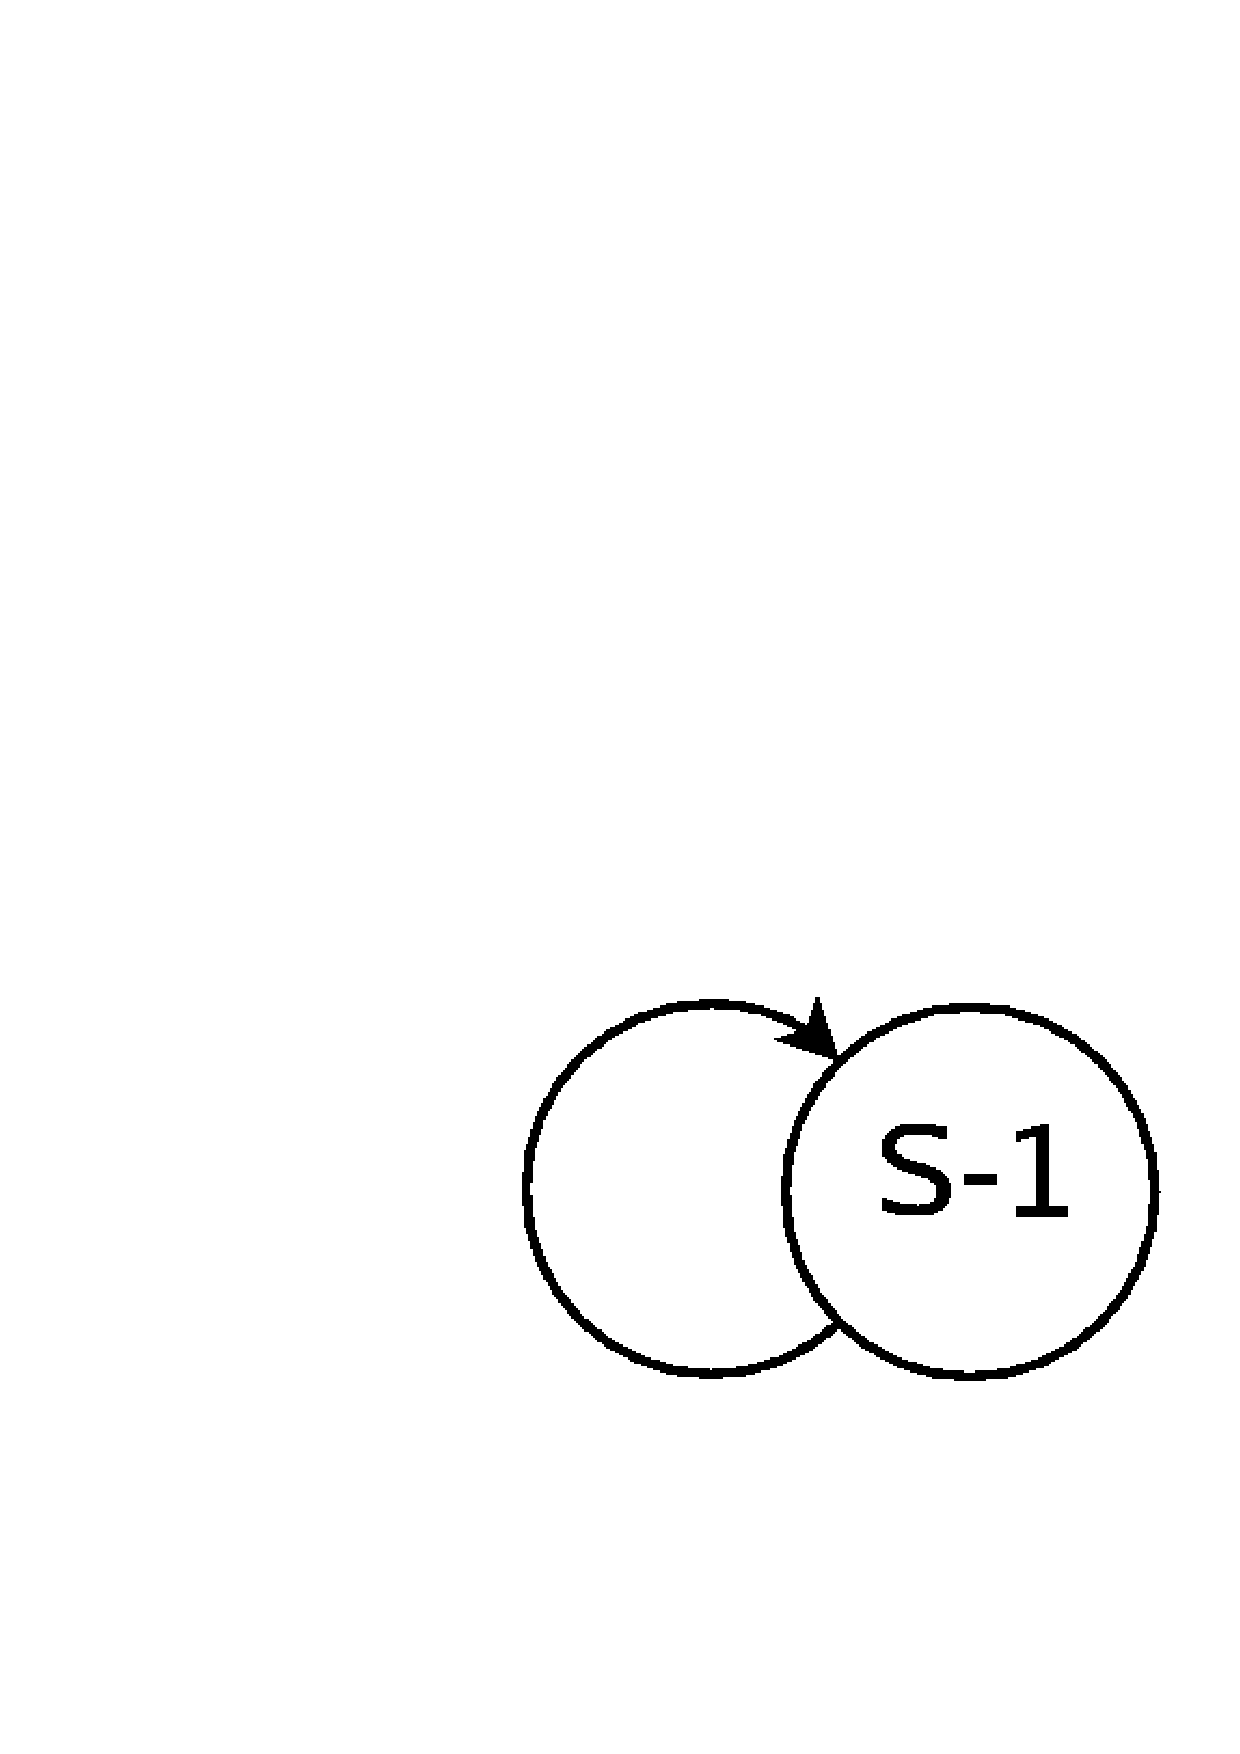
\includegraphics[width=.4\textwidth]{mutation0}
	\label{fig:ME0}
      }
      \qquad
  \subfigure
      [\mutation{AddState} mutation]
      {
	\includegraphics[width=.4\textwidth]{mutation1}
	\label{fig:ME1}
      }
      \qquad
  \subfigure
      [\mutation{AddTransition} mutation]
      {
	\includegraphics[width=.4\textwidth]{mutation2}
	\label{fig:ME2}
      }
      \qquad
  \subfigure
      [\mutation{ChangeNextState} mutation]
      {
	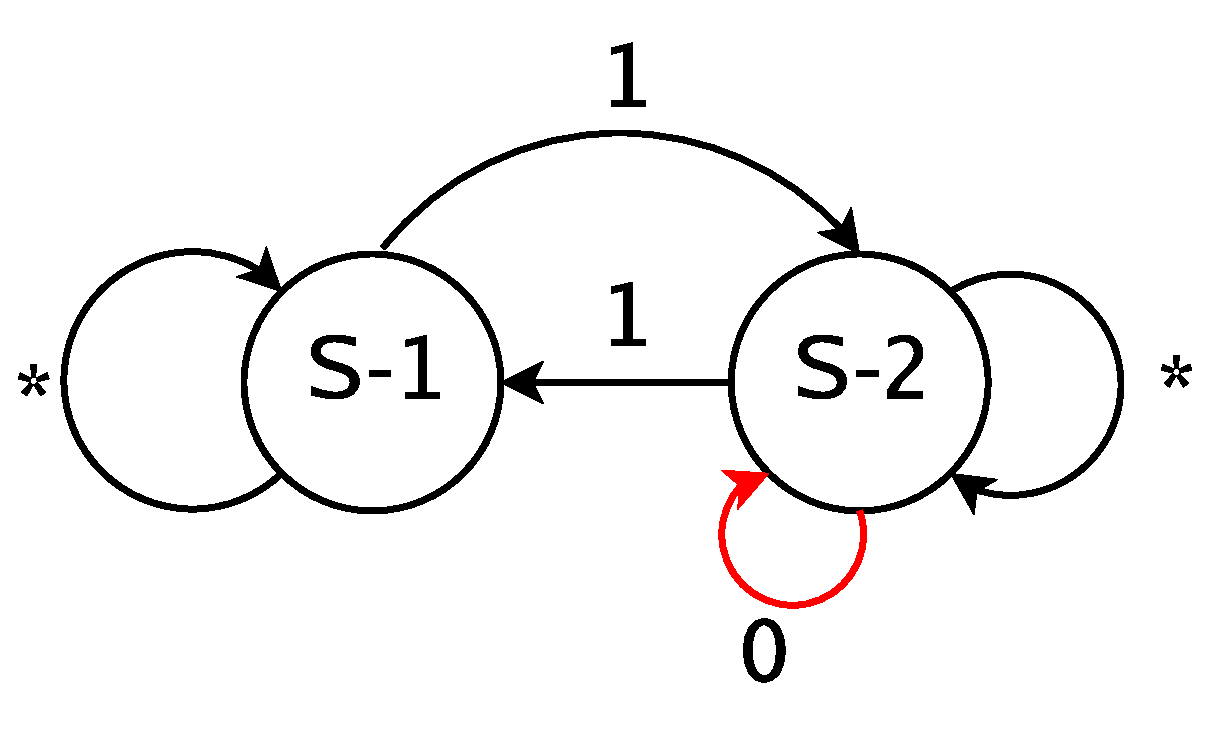
\includegraphics[width=.4\textwidth]{mutation3}
	\label{fig:ME3}
      }
      \qquad
      \centering
  \subfigure
      [\mutation{InvertSensor} mutation]
      {
	\includegraphics[width=.4\textwidth]{mutation4}
	\label{fig:ME4}
      }
      \caption[Graphical depictions of mutation operator functionality]{Graphical illustrations of how the mutation operators function.  \refFigure{ME0} shows the format of the initial state machine.  \refFigures{ME1}{ME4} successively show how each mutation affects the state machine.  Note, \mutation{ChangeAction} is not shown, but functions similarly to \mutation{ChangeNextState} by randomly selecting a transition then changing the associated action to a randomly selected action.}
\label{fig:MutationExample}
\end{minipage}
\end{figure}


\section{Fitness Evaluation}
\label{sec:fitness-function}

The driving force in an evolutionary computation system is the fitness function because it imposes an ordering on the population of solutions, with ranking determined by the aggregation of each solution's ability to satisfy some set of metrics.  Thus, the fitness function acts as a differentiator, separating the adequate solutions from the best solutions.

The idea is that the fitness function guides selection and mutation through a selective pressure that manifests through a solution's score relative to the score of the entire population.  Thus, a good fitness function filters a population on two levels: separating  \qw{bad} solutions from \qw{good} solutions, and by differentiating \qw{good} solutions from \qw{better} solutions.

Each solution in the population is a state machine that encodes the program for a single agent in a homogeneous swarm.  Thus, simulation must be used in order to evaluate the fitness of a solution.  For this work, \SWEEP is used to simulate a homogeneous swarm where each agent is programmed with the logic encoded in the state machine solution.  The simulation is then run multiple times to remove any biases introduced by the randomness of a swarm.  The fitness function takes the raw data generated by \SWEEP, which is customizable and application specific, and calculates a fitness score based on the evaluation metrics defined by the user.  In \refChapter{Results}, the specific fitness metrics used for each scenario are discussed.  

For the purpose of this work, we often normalize the fitness measure.  Thus, with normalization, the best achievable score is 1 and the worst score is 0.  Using the collection of objects as an example, say that out of 20 objects, solution $s_1$ collected 7 objects and $s_2$ collected 12.  Now say that the fitness is based solely on the number of objects collected.  Thus, the normalized fitness score for $s_1$ is $7/20=0.35$ and for $s_2$ is $12/20=0.60$.  Since the goal is to maximize fitness, $s_2$ is more fit than $s_1$.
